\documentclass[12pt,letterpaper,openright]{report}

\usepackage{amssymb}
\usepackage{booktabs}
\usepackage[T1]{fontenc}
\usepackage[margin=1in]{geometry}
\usepackage{graphicx}
\usepackage{hyperref}
\usepackage[mono=false]{libertine}
\usepackage{listings}
\usepackage{multirow}
\usepackage[numbers]{natbib}
\usepackage[libertine]{newtxmath}
\usepackage{subcaption}
\usepackage[svgnames]{xcolor}

\newcommand{\chapquotes}{}
\newcommand{\solb}[1]{{\color{magenta} TODO #1}}
\newcommand{\thesis}[1]{\solb{THESIS #1}}

\renewcommand{\contentsname}{Table of Contents}
\renewcommand{\lstlistlistingname}{List of Listings}

\lstset{captionpos=b,
	basicstyle=\ttfamily,
	keywordstyle=\color{Blue},
	commentstyle=\color{Green},
	columns=flexible,
	language=C++
}

\bibliographystyle{abbrvnat}

\newcommand{\ms}[1]{#1 ms}
\newcommand{\us}[1]{#1 $\mu$s}

\newcommand{\attribchapquote}{}
\newcommand{\widthchapquote}{}
\newenvironment{chapquote}[2][3in]{
	\renewcommand{\attribchapquote}{#2}
	\renewcommand{\widthchapquote}{#1}
	\vspace{-2in}
	\begin{flushright}
	{\Large ``}
}{
	{\Large ''} \\
	--- \attribchapquote \\
	\rule{\widthchapquote}{1pt}
	\end{flushright}
	\vspace{1in}
}

\makeatletter
\let\includegraphics@\includegraphics
\renewcommand{\includegraphics}[2][]{\includegraphics@[#1]{\includegraphicsdir#2}}
\newcommand{\includegraphicsdir}{}

\let\input@\input
\renewcommand{\input}[2][.]{
	\renewcommand{\includegraphicsdir}{#1/}
	\input@{#1/#2}
	\renewcommand{\includegraphicsdir}{}
}

\let\section@\section
\newenvironment{swallowsections}{
	\renewcommand{\section}[1]{}
}{
	\let\section\section@
}
\makeatother

\renewenvironment{abstract}{}{}

\newcommand{\mytableistoobig}{}

\begin{document}

\begin{titlepage}
\begin{center}
	\vspace*{\fill}

	\textbf{\Large Lightweight Preemptible Functions} \\
	A thesis \\
	\hfill \\
	{\large Sol Boucher} \\
	\today \\

	\vspace{1in}

	\textbf{Thesis committee:} \\
	David G.\@ Andersen, \textit{chair} \\
	Adam Belay \\
	Michael Kaminsky \\
	Brandon Lucia \\

	\vspace{\fill}

	\textit{Submitted in partial fulfillment of the requirements \\
	for the degree of Doctor of Philosophy} \\
	\hfill \\
	Computer Science Department \\
	School of Computer Science \\
	Carnegie Mellon University \\
	Pittsburgh, PA 15213 \\
\end{center}
\end{titlepage}

\pagenumbering{roman}
\tableofcontents
\listoffigures
\listoftables
\lstlistoflistings
\newpage
\pagenumbering{arabic}

\chapter*{TODOs THESIS}

\section{POSIX contexts self-signaling trick (897fe6b)}

The handler's logic is as follows:  It checks whether
the preemptible function has exceeded its timeout; if so, it swaps the contents
of the signal handler's continuation (accessible via the final argument to the
function~\cite{sigaction-manpage}) with a checkpoint continuation saved by
\texttt{launch()}.  This causes the subsequent return from the signal handler
to jump back to \texttt{launch()}, which then returns a \texttt{linger}
structure containing the signal handler's original context.  A subsequent
\texttt{resume()} call on this packaged continuation proceeds in much the same
way as \texttt{launch()}, but resumes the original computation by sending
itself a special signal with \texttt{pthread\_kill()}, then swapping the saved
context with the contents of that handler's context\footnote{This is necessary
because POSIX left the semantics of calling \texttt{setcontext()} on the
continuation saved by a signal handler invocation unspecified, leading
implementations such as GNU not to handle this
case~\cite{getcontext-manpage}.}.

Signal pool trick:\@ see 17b86d2.


\section{Cross-library symbol detection algorithm (7aa3541)}

Identifying which GOT entries correspond to cross-library symbol uses
is is a multi-step process:
First, we traverse the relocation table for each loaded object file, cross
referencing each of its relocation entries against the local object file's symbol
table.  If the symbol table does not contain a definition matching the relocation
entry's target, we conclude that the relocation must correspond to a cross-library
call.  Otherwise, we check the address in the GOT entry corresponding to the
relocation entry:  If this address is outside the bounds of the current object file,
it is a cross-library call.  Otherwise, if this address matches the one from the
symbol table entry, it is not a cross-library call, and should be skipped.  The last
case is the trickiest, since the GOT entry probably still refers to the PLT stub
(because the symbol reference has not yet been resolved).  In this case, we resolve
the symbol
early, update the GOT entry, and recheck whether it resolved to the local definition
to determine whether it is a cross-library call.


\section{ELF \textit{NODELETE} dynamic flag workaround (8dcf62b)}

Some shared libraries are marked with a special configuration flag,
\texttt{DF\_1\_NODELETE}, which prevents the dynamic linker from ever removing them
once they have been loaded.  Because almost all libraries depend on libc, the
presence of even one such library prevents us from reinitializing a libset for reuse
after its preemptible function has been canceled!  The flag is mostly used on
libraries that need
to monkey-patch some other loaded library, such that the two subsequently have a
circular dependency.  Fortunately, this is not usually a problem because when we
unload one library from a libset, we then unload the rest, so whenever we encounter a
\texttt{NODELETE} object file, we make a special copy with the flag cleared, for
loading into every namespace except the main one.  The one place this does not work
is when a library monkey-patches the dynamic linker itself.  This
requires the use of a private interface, and the only offending library to our
knowledge is GNU libpthread, which replaces function pointers in order to cause the
dynamic linker to take locks when performing potentially concurrent operations; we
handle this by preventing the monkey-patching constructor code from running in our
modified copy of that library.


\section{Preserving pointer equality (5d4b902)}

A subtle but important point in the semantics of dynamic linking is that pointers to
the same definition must compare equal, regardless of where they are obtained.  For
instance,
the reader might notice that invocation is not the only thing a program can do with a
function:\@ it might also pass around the function's address.  In fact, after taking
the address, it could pass it to code within a different object file, which might
compare it\footnote{In order for such comparisons to correctly indicate whether the
same code will be run, the compiler loads such addresses directly from the GOT via
instructions of the special position-independent relocation form
\texttt{mov~\textit{symbol}@gotpcrel(\%rip),~\%\textit{dest}}, and the dynamic linker
resolves the calls and populates their GOT entries eagerly at load time.}.  To avoid
breaking pointer comparison, libgotcha makes sure to share the same PLOT
stub between all GOT entries to a given symbol that use this type of
relocation.  As long as the current libset remains the same between the time of a
function pointer comparison and the time of its invocation, such a comparison
guarantees that \texttt{procedure\_linkage\_override()} will dispatch to the same
copy when invoked using either pointer.


\section{Lazy PLT relocation memoization trick (154d76e)}

The setup procedure described so far has one significant problem:\@ recall that a PLT
call memoizes the real address of its symbol by replacing the GOT entry, which should
cause subsequent calls to skip libgotcha's \texttt{procedure\_linkage\_override()}
codepath.  In order to prevent this, the constructor updates the relocation entries
corresponding to cross-library calls to point at \textit{shadow} GOT entries.  This
fools the dynamic linker into updating the shadow entry instead, meaning that
memoization still works, as shown in Figure~\ref{fig:override}.

\begin{figure}
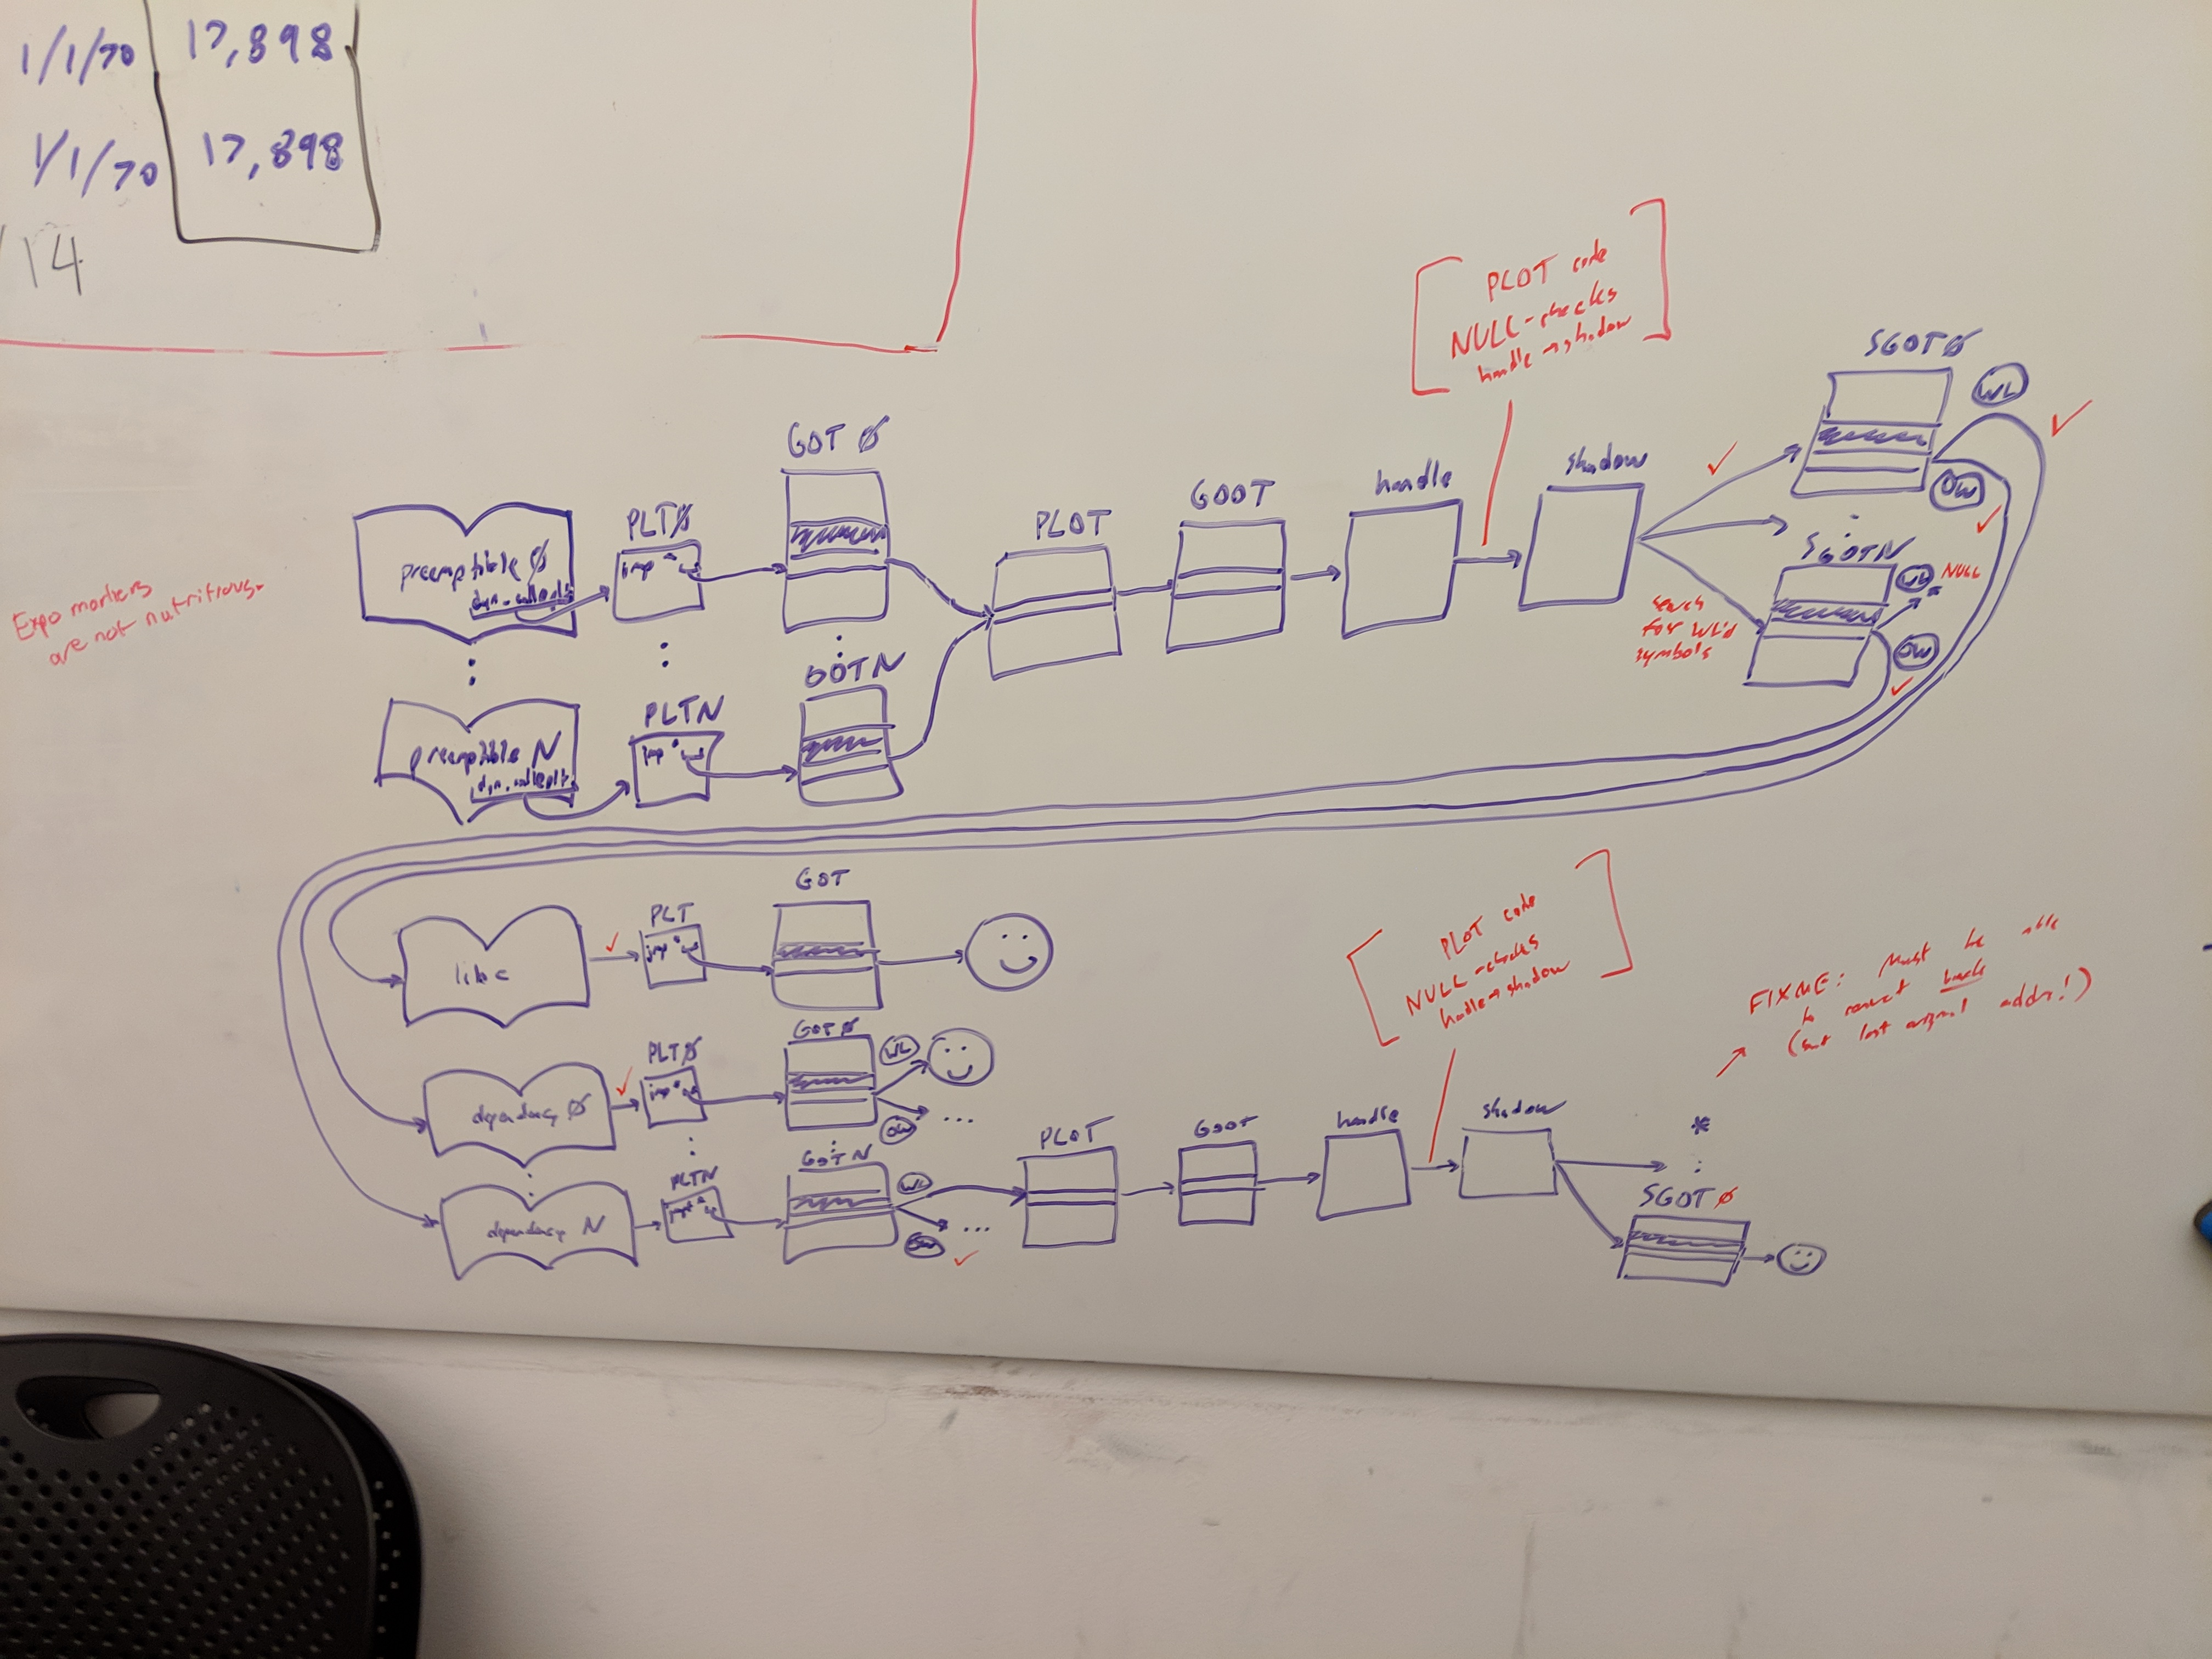
\includegraphics[width=\columnwidth]{functions/figs/tables}
\caption{\texttt{procedure\_linkage\_override()} tables}
\label{fig:override}
\end{figure}


\section{Global variable interception heuristics (gotcha ebef4e0)}

Woah!  The error was in executing this instruction, which probably means it's
unreadable.  Let's *not* try to disassemble it; instead, we'll see whether we
just followed a misguided indirect call instruction.  First search backward from
the return address for such an instruction...

It looks like the base of the displacement-mode address calculation isn't one we
instrumented.  Maybe the code computed a custom base address using a register
that we've since updated due to a separate (but nearby) dereference?

See whether we can apply one of our heuristics.  Note that they currently assume
that the code applied a *linear* offset to the last address we resolved.

Let's try adding the same offset we did last time we resolved an address,
because we're in one of the following common situations:
\begin{itemize}
\item The client code is using the same base address register as it was
	during our last trip through this function.  This might indicate that
	said code is using the register as an address accumulator, but doing
	so in concert with some other temporary register: because of this
	indirection, overwriting the register with the temporary after we
	had preformed the original address resolution would have left us
	unable to process any subsequent values accumulated into the register.
\item The base address register is different than the one updated during our
	last trip through this function, but the value of the latter has
	remained unchanged since we updated it.  Because it contains a memory
	address we had to resolve, this strongly suggests that the client code
	has only executed a few instructions since then, which we can infer
	even if that set included one or more branch instructions.
\item The current return address points to the instruction immediately
	following the one that faulted to result in the last invocation of
	this function, and the current base address register's value has
	remained the same since the faulting instruction was executed.  This
	implies that said instruction was an indirect procedure call, and that
	the register was probably just used to pass a pointer argument.
	Because we didn't resolve the address of the indirect call until the
	client code was already transferring control, there was no way for it
	to have passed a pointer without performing arithmetic directly on the
	dummy address present before the call.
\end{itemize}

We resolved the address without applying a heuristic.  Save a record of what we
changed and how to allow us to heuristically resolve addresses based on our
experience.  Because this is guarded, heuristics cannot chain, but multiple of
them can be triggered based on a common base resolution.


\section{Uncopyable function calls diagram (424387e)}

See Figure~\ref{fig:uncopyable}.

\begin{figure}
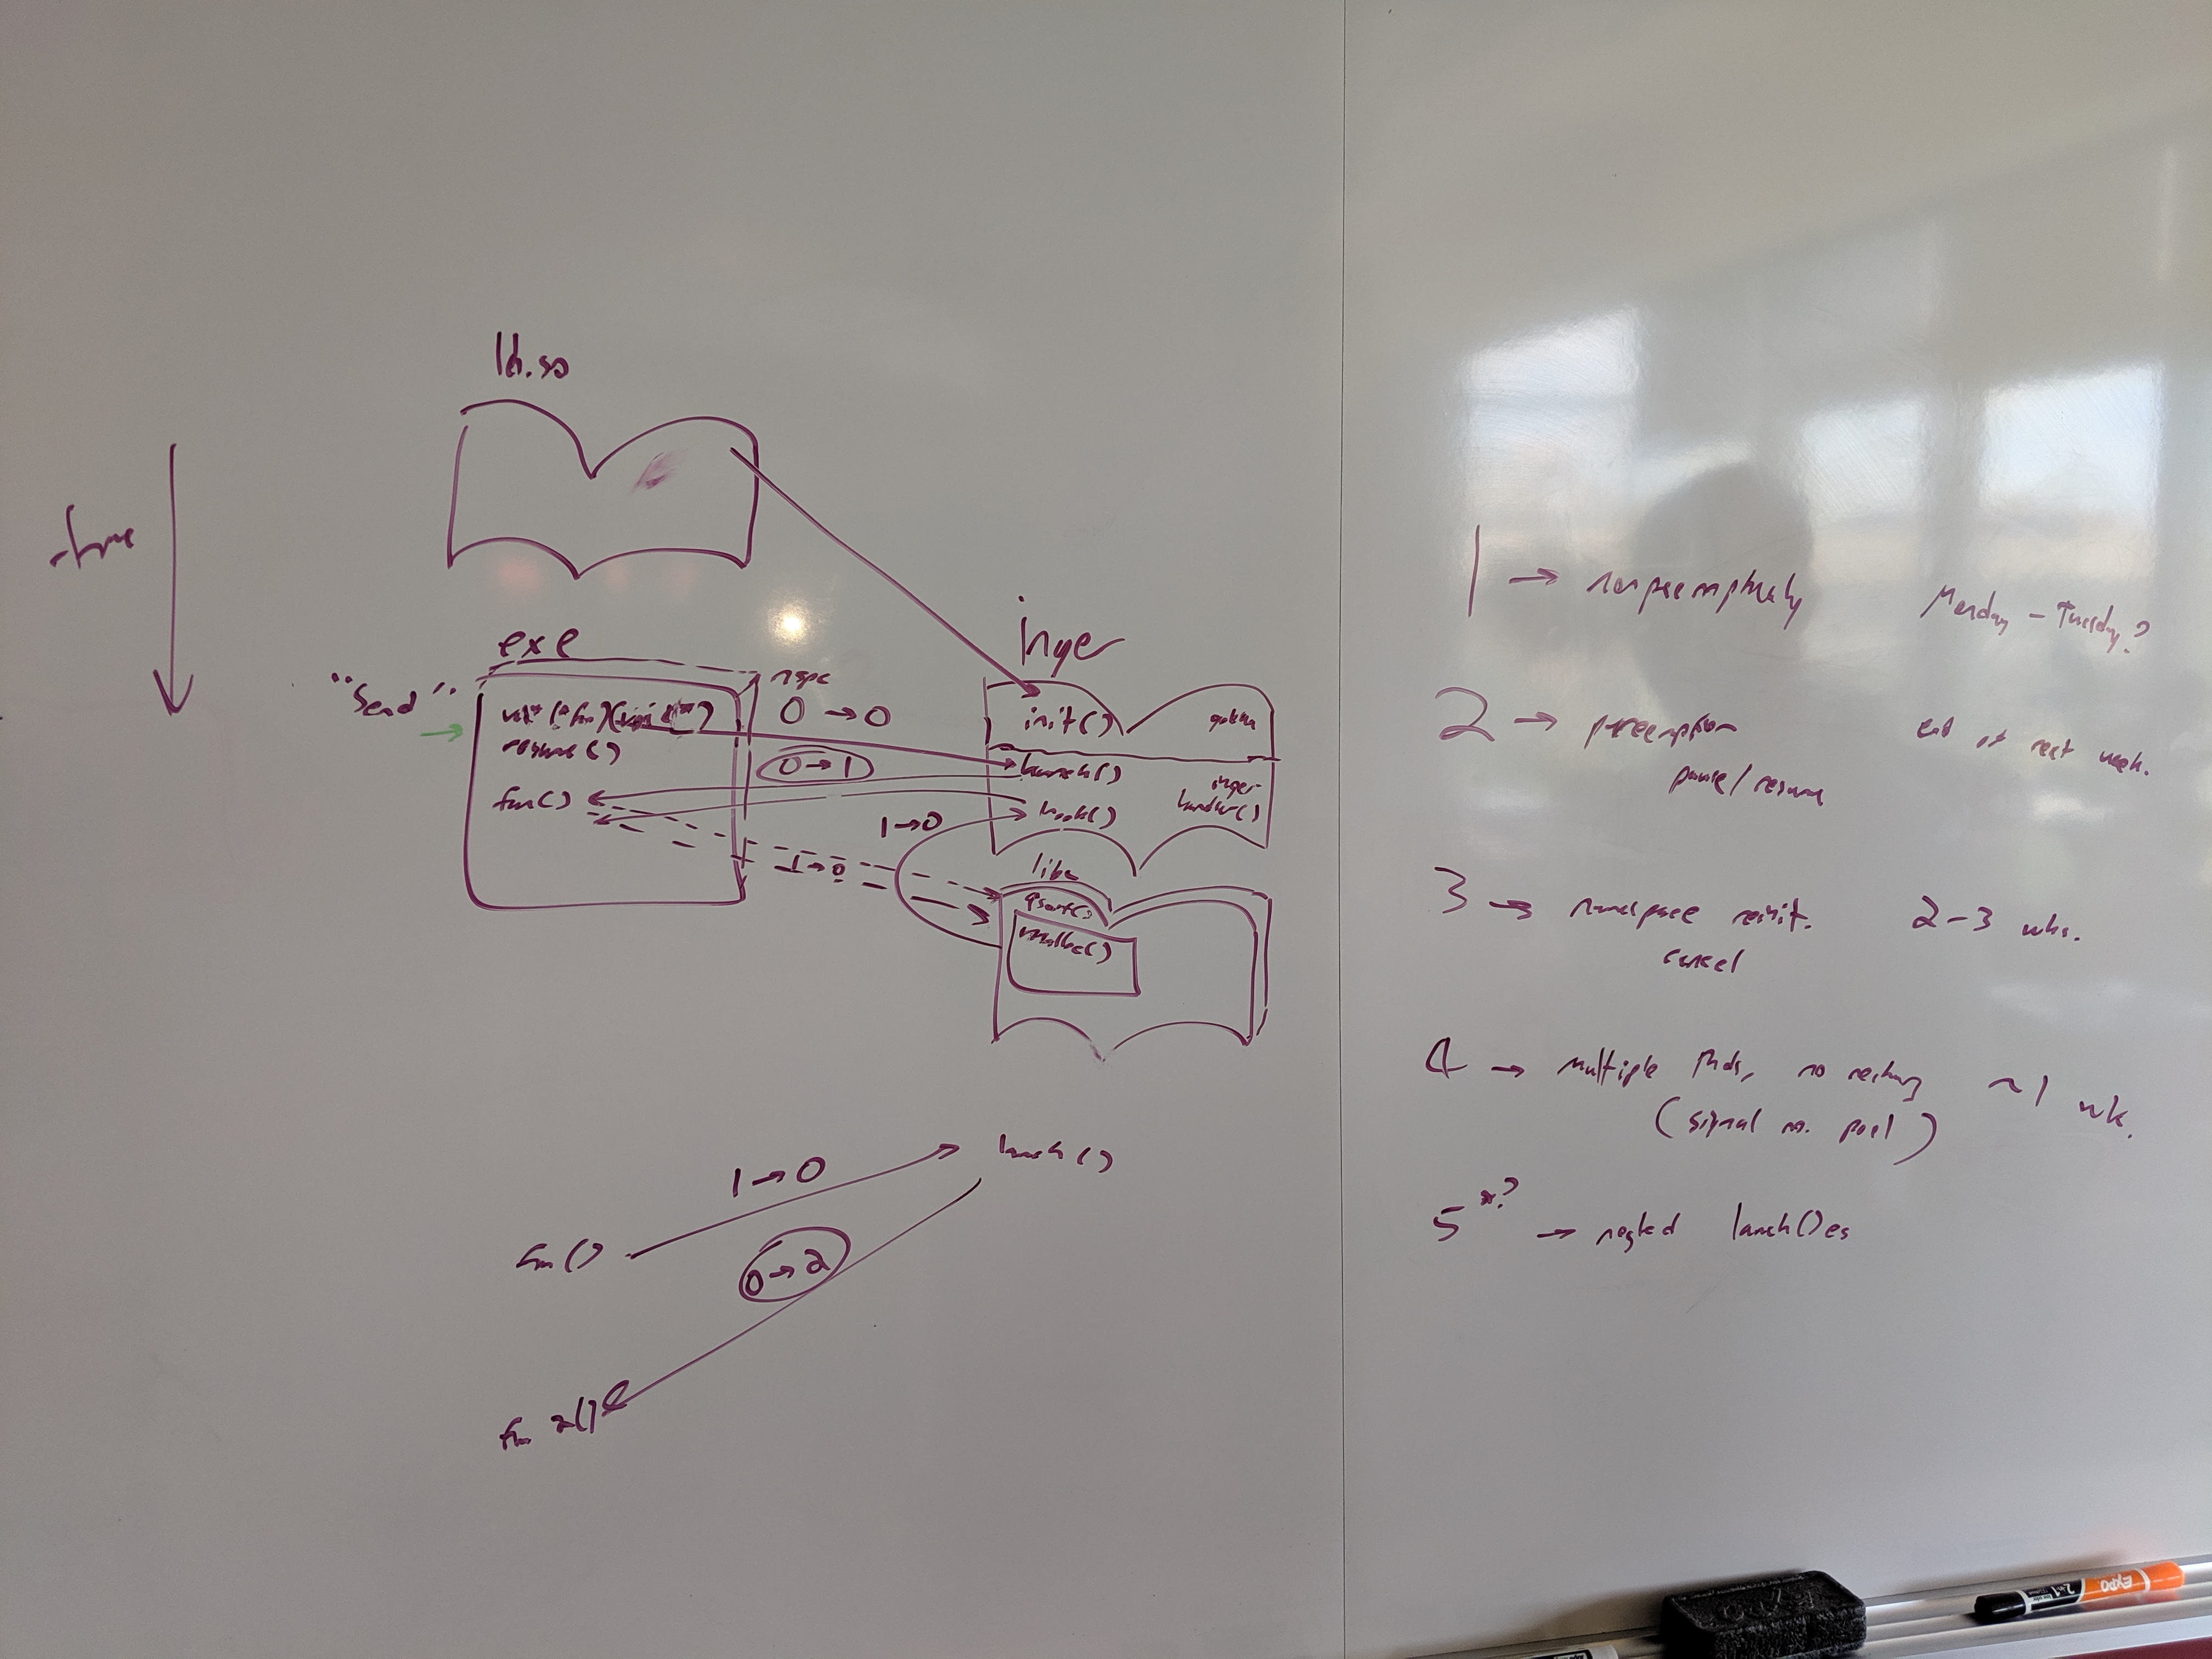
\includegraphics[width=\columnwidth]{functions/figs/calltree}
\caption{What happens when a program calls an uncopyable function}
\label{fig:uncopyable}
\end{figure}


\section{Program automatically repaired by libas-safe (ee2602a)}

The main use of libgotcha is to make library function calls async-signal safe when
they would not otherwise be.  To more clearly illustrate the library's usefulness, we
pause to give a minimal example of such usage; specifically, we will leverage
libgotcha to automatically fix the buggy program in Listing~\ref{lst:handlerbug},
which calls the async-signal-unsafe function \texttt{printf()} from its signal
handler.  Unfortunately, this function takes a lock on the \texttt{stdout} stream's
associated file descriptor, and the signal handler eventually interrupts the program
within \texttt{fflush()} while it is holding this same lock, resulting in deadlock.

\begin{figure}
\begin{lstlisting}[label=lst:handlerbug,caption=C program with a buggy signal handler]
static void handler(int ignored) {
  printf("In signal handler\n");
}

int main(void) {
  struct sigaction sa = {
    .sa_handler = handler,
  };
  sigaction(SIGALRM, &sa, NULL);

  struct timeval tv = {
    .tv_sec = 1,
  };
  struct itimerval it = {
    .it_interval = tv,
    .it_value = tv,
  };
  setitimer(ITIMER_REAL, &it, NULL);

  while(true)
    fflush(stdout);
}
\end{lstlisting}
\end{figure}


\section{Footnote introducing the concept of libac-safe (d3336e4)}

While libas-safe reestablishes async-signal safety, it would also be
possible to write a libgotcha client library that did the same for what POSIX calls
async-cancellation safety.  The obvious application of this would be supporting
asynchronous thread cancellation (in the common case where whitelisted code was not
currently executing):\@ as we saw in Section~\ref{sec:intro}, today's POSIX and
Windows interfaces for this are broken to the point of practical uselessness.


\section{Process image diagrams}

Per module (Figure~\ref{fig:procimgobj}) and per thread (Figure~\ref{fig:procimgthd})

\begin{figure}
\includegraphics[width=0.6\columnwidth]{figs/procimg_perobj}
\caption{Per--object file portion of process image}
\label{fig:procimgobj}
\end{figure}

\begin{figure}
\includegraphics[width=\columnwidth]{figs/procimg_perthd}
\caption{Per-thread portion of process image}
\label{fig:procimgthd}
\end{figure}


\section{Libset reinitialization diagram}

See Figure~\ref{fig:reinit}.

\begin{figure}
\includegraphics[width=\columnwidth]{figs/reinit}
\caption{Libset reinitialization to support asynchronous cancellation}
\label{fig:reinit}
\end{figure}


\section{Preemptible functions rebuttal}

\input{functions/rebuttal/atc20-reviews-198.txt}


\section{A note on terminology (inger 7d5b2e2)}

We use the term lightweight preemptible function (LPF) to refer to the timed \textit{version} of a
function, as invoked via the \texttt{launch()} wrapper function in this library.  It's not quite right to
say that \textit{libinger} "provides preemptible functions"; rather, it provides a transformation from
an ordinary function into a preemptible one.

To provide the memory isolation necessary to introduce preemption and asynchronous cancellation at
sub-thread granularity without breaking existing program dependencies, the \textit{libgotcha} runtime
allocates a separate copy of all the program's loaded dynamic libraries for each preemptible
function.  While the paper refers to this isolation unit as a libset, that term was unfortunately
coined late in development; as such, the source code and configuration variables refer to it as a
"group" instead.


\section{A note on design (inger 7d5b2e2)}

The paper describes the \textit{libinger} API, and the generated HTML documentation gives a few more usage
details.  Here are some of the guiding principles that inspired our interface choices:
\begin{itemize}
\item **We do not assume users need asynchrony.**  Hence, preemptible functions \textit{run on the same kernel
	thread as their caller}.  This is good for performance (and especially invocation latency), but
	it is also important to be aware of; for instance, it means that a preemptible function will
	deadlock if it attempts to acquire a lock held by its caller, or vice versa.  If asynchrony is
	something you require, you can build it atop \textit{libinger}, as we have demonstrated with our
	\textit{libturquoise} preemptive userland thread library.
\item **We assume that simply calling a function with a timeout is the common use case.**  As such, the
	\texttt{launch()} wrapper both constructs and begins executing the preemptible function rather than
	asking the user to first employ a separate constructor.  The latter behavior can be achieved by
	passing the sentinel \texttt{0} as the timeout, then later using \texttt{resume()} to invoke the preemptible
	function.
\item **We endeavor to keep argument and return value passing simple yet extensible.**  Because Rust
	supports closures, the Rust version of \texttt{launch()} accepts only nullary functions: those seeking
	to pass arguments should just capture them from the environment.  Because C supports neither
	closures nor generics, the C version of \texttt{launch()} accepts a single \texttt{void *} argument that can
	serve as an inout parameter; it occupies the last position in the parameter list to permit
	(possible) eventual support for variable argument lists.
\item **We choose defaults to favor flexibility and performance.**  When a preemptible function times
	out, \textit{libinger} assumes the caller might later want to resume it from where it left off.  As
	such, both \texttt{launch()} and \texttt{resume()} pause in this situation; this incurs some memory and time
	overhead to provide a separate execution stack and package the continuation object, but has much
	lower overall cost than asynchronous cancellation.  If the program does require cancellation, it
	can request it explicitly by calling \texttt{cancel()} (C) or dropping the continuation object (Rust).
\item **We provide preemption out of the box, but the flexibility to cooperatively yield.**  The
	\texttt{pause()} primitive allows a preemptible function to "yield" back to its caller by immediately
	"timing out."  One can imagine building higher-level synchronization constructs atop this; for
	example, a custom mutex that paused instead of blocking would allow two or more preemptible
	functions to share state, even when some of them executed from the same kernel thread.
\item **We favor a simple, language-agnostic interface.**  Because the interface is based on the
	foundational function call abstraction, it looks very similar in both C and Rust.  Someday, it
	may look \textit{equally} similar in other languages as well, and in the meantime, it ought to enjoy
	compatibility with languages' C foreign-function interfaces.  It's relatively simple to integrate
	higher-level abstractions on top, such as the Rust futures wrapper available in \textit{libinger}'s
	\texttt{future} module.
\end{itemize}


\section{A note on implementation (inger 7d5b2e2)}

The timer signal handler in \textit{libinger} refuses to pause while the next libset is set to 0 (the
starting libset).  Because \textit{libinger} is statically linked with \textit{libgotcha}, the latter enforces a
transparent switch to this libset whenever a dynamic function call transfers control into the module
in the process image that corresponds to \texttt{libinger.so}.  This means that preemption is deferred on a
given kernel thread while \textit{libinger}'s own code is executing on that thread.

Of course, things are not quite that simple.  There are noteworthy exceptions to the rule:
\begin{itemize}
\item The public \textit{libinger} Rust interface includes a number of generic functions.  Because the Rust
	compiler monomorphizes such functions for the client code that uses them, \textit{their implementations
	are \textrm{not} in \texttt{libinger.so}!}  Rather, there is, roughly speaking, one or more copies of them
	(specialized for various type arguments) in each program module that calls them.  The generic
	functions are therefore implemented such that they package everything that differs by type, then
	call into non-specialized functions such as \texttt{setup\_stack()} and \texttt{switch\_stack()} to do the scary
	stuff.
\item The \texttt{resume\_preemption()} function is installed as a \textit{libgotcha} callback hook, and is implicitly
	invoked at the end of each deferred-preemption library call made by a preemptible function.
	\textit{This happens in the preemptible function's libset rather than the starting one}; this is
	essential because the callback's main task is to force the timer signal handler to run
	\textit{immediately} and check for a timeout, and we don't want the libset to inhibit preemption!
\end{itemize}


\section{Building glibc from source (inger 7d5b2e2)}

Although \textit{libinger} is compatible with an unmodified glibc in principle, in practice the build
configuration used by most distributions is insufficient for two reasons:
 * By loading numerous copies of the application's libraries, we tend to exhaust the static storage
   pool provided by the dynamic linker.  If your program hits this limit, it will crash at load time
   with an error like: \texttt{yourprogram: libgotcha error: Unable to load ancillary copies of library:
   somelibrary.so: cannot allocate memory in static TLS block}.
 * Stock glibc builds are limited to 16 linker namespaces, enough to support only 15 preemptible
   functions at any given time.  If your program hits this limit, it will crash at runtime with an
   error like: \texttt{launch(): too many active timed functions}.

Unfortunately, these configuration parameters are baked into the dynamic linker at build time.
What's more, changing (at least) the latter alters the size of internal structures that are shared
between \texttt{ld-linux.so}, \texttt{libc.so}, \texttt{libpthread.so}, and others, so making changes requires rebuilding
all of glibc.  Fortunately, provided you set the prefix properly when building glibc, the dynamic
linker will know where to search (by absolute path) for the other libraries; as such, most
applications that depend on \texttt{libinger.so} need only define a custom interpreter path pointing to the
\texttt{ld-linux-x86-64.so.2} file in your build directory.


\section{Control libraries (gotcha 8224235)}

There are two possible types of control library:
\begin{itemize}
\item An \textit{internal control library} is statically linked with \textit{libgotcha} to form a single shared
   object file that is loaded (or preloaded) as one unit.  In addition to having access to the
   \textit{libgotcha} control API (declared in \texttt{libgotcha\_api.h}), internal libraries enjoy the guarantee
   that their code always executes in the base libset, and have direct access to the C library
   functions deemed by \textit{libgotcha} to be too dangerous for the rest of the program to call
   (enumerated in \texttt{libgotcha\_repl.h}).
\item An \textit{external control library} is dynamically linked with \textit{libgotcha}, and therefore constitutes
   a separate shared object file that depends on \texttt{libgotcha.so} (or, perhaps, a compatible internal
   control library).  Calls into such a library do not cause an automatic libset switch unless
   explicitly whitelisted (which is currently not pluggable and done via \texttt{whitelist.c}), and the
   library does not have special access to dangerous C library functions.  External control
   libraries haven't been tested as extensively as internal ones, but are necessary when you want to
   have more than one control library in a single application, if you want to be able to update
   \textit{libgotcha} without rebuilding the control library, and maybe for other reasons yet to be
   discovered.
\end{itemize}

If an internal control library needs to alter the behavior of any additional third-party library
functions, it may designate them as dangerous by defining its own implementation of the same name.
Calls to the function from the rest of the process image will be rerouted to this implementation,
but calls from the control library (and \textit{libgotcha} itself) will be routed to the original
third-party implementation.  For more details, see the documentation in \texttt{libgotcha\_api.h}, the
advice about compiler optimizations in \texttt{libgotcha\_repl.h}, and the example control libraries in the
projects under the \texttt{example} directory.

Note that internal control libraries' calls to \textit{existing} dangerous C library functions are also
routed directly to the real implementation, but the control library may instead choose to call
\textit{libgotcha}'s safer wrapper.  A control library might even use this feature to wrap \textit{libgotcha}'s
own wrapper of a third-party library function!  These use cases are considered advanced: see the
documentation in \texttt{libgotcha\_repl.h}, and be prepared for some additional build system complexity
(e.g., our Make integration supports replacing calls to \texttt{cp} via the \texttt{\$(CP)} variable, which could
be used to inject an intermediate \texttt{objcopy} step into the build process).


\section{Lessons for system builders (slides)}

Resuming is a useful feature that is cheap, but introduces concurrency.
Cannnot get CPU time isolation without memory isolation.
Design abstractions modularly and with an eye to simple use cases (e.g., libgotcha as a separate
runtime with a very small control API, things listed in the note on design).
Treat debuggability as a first-order concern (e.g., permit disabling features that interfere at
runtime, test and maintain support for running under debugging and diagnostic tools).


\chapter*{Foreword}

Perhaps it is inevitable that when a nonfiction work reaches a certain length, it
begins to serve multiple purposes; if so, this document is no exception.  Yes, it is
a record of the ideas I have explored over the past years of my life.  But like any
thesis, it is also a lesson:\@ in summarizing my findings from these explorations, it
endeavors to save you from spending years of your own on the same topic.  And like
any good lesson, this one begins with an exercise...

With your permission, we will conduct a brief mindfulness activity.  At this moment,
and for however much longer you focus on this document, you mind will be occupied by
ideas.  Many of these ideas I will have put there.  Shortly, they will be ideas about
computer systems, but first let us consider:  How are the ideas getting to you?  You
are reading, but what does that mean?  Perhaps you are holding a printout or a bound
copy of this manuscript, or perhaps you have loaded it onto your personal computer,
tablet, phone, or hand terminal.  In any case, you have opened it to a particular
page, exposing your eyes to a sea of shapes arranged into nested clusters.  Your eyes
have gravitated to a cluster of particularly large shapes known as a ``chapter
title,'' then they have scanned across the page and sent a compressed representation
of each smaller ``word'' cluster of shapes to your brain, which has matched the
clusters of shapes to entries in your mental lexicon, then parsed them according to a
set of linguistic rules to infer their logical connections.  Then you have moved on
to the large ``paragraph'' clusters and processed each in turn, starting with the
first of its ``sentence'' clusters, and in so doing, learning what the next sentences
will be about.  Occasionally, something will go wrong at one of these steps and you
will backtrack and notice a missed word, or more closely examine a misidentified
word, or try a different parsing of the sentence, or reexamine the logical flow of
the paragraph.  You will usually not realize you are doing any of this, preferring
to think simply that you are \textbf{reading}.

The document you are reading is about computer systems, and like your brain, such
systems have many complexities.  If we as computer users had to describe the full
process for doing everything, we would never accomplish anything, so instead we
build \textbf{abstractions} for performing common tasks without examining the
underlying details.  Some would say that any computer systems research is
fundamentally about abstractions.  This particular work centers around an abstraction
for use by application programmers, who in turn work on top of other abstractions,
the most notable of which is software called the \textbf{operating system}.

In computing, as in life, one's fundamental goal is to accomplish some task using a
set of shared resources.  Someone must decide how to allocate these shared resources,
a role usually filled for a particular resource by a piece of software called its
\textbf{scheduler}.  One major responsibility of the operating system is to share
hardware resources such as the processor, the short- and long-term storage devices,
devices for user interaction, and network interfaces.  Among these, the one most
relevant to our discussion is the CPU scheduler, which manages the processor.

Despite itself being an abstraction that hides enormous complexity, a processor is
conceptually quite simple:\@ it receives a stream of simple \textbf{instructions}
telling it what to do, executing them in the order received and occasionally jumping
to a particular point elsewhere in the stream when so instructed.  The simplicity of
this model belies the infinite expressive power of programs constructed from such
instructions.  Indeed, programming at the instruction level is difficult not only
because the simplicity of the instructions make it verbose, but also because ad-hoc
jumps can be deceptively complicated to reason about.  Modern programmers usually
write software in programming languages that provide so-called ``structured control''
abstractions for performing common, formulaic sequences of jumps.

The most fundamental abstraction composing a structured program is the
\textbf{function}:\@ a section of code that expects zero or more input data, performs
some computation, and generates zero or more output data.  One function can call
another, which automatically transfers the input data and jumps to the start of that
function's code.  Later, when the end of its code is reached, the function
automatically jumps back to the program point just after it was called and transfers
its output data back.  Notice that a function call is \textbf{synchronous}; that is,
the function runs to completion before the calling function continues to run.
Because such sequential execution matches the processor's inherent behavior, sharing
the processor between functions is trivial and requires no scheduler.

Of course, an important feature of modern computers is the ability to work on
multiple tasks alongside each other, such as reading a document and composing an
outline or notes.  Operating systems manage such situations by providing an
abstraction called a \textbf{process}, or independent task.  Each process is isolated
from the others on the system and cannot access their data.  Furthermore, processes
exhibit a property known as \textbf{concurrency} wherein their executions can
interleave such that one process executes some of its code ``in the middle of''
another process's work.  (Think of momentarily putting your notetaking on hold to
scroll down in the document you're reading.)

Because isolation prevents processes from calling each other's functions directly,
switching between processes requires a scheduler to transfer control of the
processor.  Specifically, the processor must stop executing the running process and
start running the operating system's CPU scheduler code, which then performs an
action called a \textbf{context switch}:\@ it saves a checkpoint of that process and
restores the other process, resuming it from the state in which it last left off.
The conceptually simpler way for this transition to happen is \textbf{cooperative}
multitasking, in which the former process voluntarily gives up control of the
processor by explicitly telling the operating system to give someone else a turn.
Unfortunately, it is not safe to assume a process will eventually cede its processor,
as it may never decide to do so, through either misbehavior or malice.  Such a
scenario would render the rest of the programs unusable.

Fortunately, processors have a low-level mechanism for spontaneously changing which
instruction they are executing known as a \textbf{timer interrupt}.  Every so often,
the processor jumps into the OS scheduler from whatever code it is currently
executing.  Since it is now has the use of the processor, the scheduler can decide
whether to jump back to that same program or context switch to a different one, a
decision that is usually made based on how long the former program had been running
since the last context switch.  This style of process scheduling is known as
\textbf{preemptive} multitasking because the operating system initiates it by
actively pausing the running process.

Recent decades have seen the introduction of multicore computers that have more than
one processor, creating the opportunity for the operating system to schedule a
different process on each.  Such processes exhibit \textbf{parallelism}:\@ they
actually run at the same time.  Parallelism is also an attractive feature for
application programmers because by carefully restructuring their programs, they can
route some of their work to each processor, thereby speeding up portions of their
program's run.  Unfortunately, fitting such programs into operating systems' existing
process model was cumbersome.

To better accommodate parallel programs, operating systems introduced a hybrid
abstraction called a \textbf{thread}.  Like processes, threads can be both concurrent
and parallel.  Unlike processes, though, threads must share data to effectively
work together on a single task, so the threads within a process are not isolated from
one another.  It turns out that the simultaneous presence of concurrency and shared
data introduces fundamental challenges that make it difficult to write correct
programs due to a class of bugs informally known as race conditions.  Although safe
concurrency is a popular area of study, challenges remain particularly in systems
containing components that predate the parallel programming paradigm.  More detailed
coverage of safe concurrency and backwards compatibility as they relate to this
thesis work appears in chapters~\ref{chap:libinger} and \ref{chap:libgotcha},
respectively.

The lack of isolation between threads permits the programmer to spawn a thread in
much the same way they would call a function:\@ in most programming languages, they
place the code they want to execute on the new thread in its own function, but
instead of calling it directly, they pass it to a special wrapper function.  The
wrapper sets up the thread and begins running the programmer's custom thread thereon.
However, in an important break from functions, threads are \textbf{asynchronous} like
processes.  The wrapper function returns almost instantly, even if the thread is
still running in the background.  As with processes, this property means there must
be a scheduler to decide which application code each processor should run.  Note
that for the sake of this discussion, we are assuming this is the operating system's
CPU scheduler; however, this is not always the case and sometimes a custom scheduler
runs as part of the application itself, a configuration that is addressed in detail
in chapter~\ref{chap:libturquoise}.

Introducing additional scheduler dependencies on an application has important
functionality and performance ramifications for two fundamental reasons.  First, the
scheduler's placement behind an abstraction decouples it from the program's logic,
thereby imposing one or more levels of communication barrier that reduce its
understanding of the particular application's needs, often resulting in a brittle
policy ill suited to the workload.  For instance, few preemptive schedulers provide a
way for an application to customize the timer interrupt interval, even when supported
by the hardware.  Second, every scheduler works by running its own code to make
decisions about how to allocate a resource.  Because it does not represent useful
work from the application's perspective, time spent this way is pure overhead, and it
follows that introducing unnecessary scheduling necessarily reduces performance.

Threads represent the standard application for exploiting preemption within an
application.  However, reminiscent of how processes were cumbersome to use for
parallel programming, threads are ill suited to some use cases of preemption.  For
one thing, programmers who do not need parallelism are led to build their synchrony
atop asynchrony, thereby introducing a useless scheduler dependency.  For instance,
when calling a helper function but needing a result by a specific deadline is tempted
to spawn the function on its own thread, then immediately wait for the thread to
finish, a task better accomplished on the same thread.  Furthermore, although they
support pausing code mid-execution, threads make it very difficult to cancel
in-progress work that is no longer needed at all.

Fortunately, the tendency to use threads for application-level preemption is not
because the operating system does not expose hardware features such as timers.
Rather, it is because such features are presented as very low-level abstractions that
perform hardware-style unstructured jumps rather than using language-style structured
control and abstracting away the details of context switching.  We therefore propose
a new abstraction for easy preemption within an application, but show that it can be
implemented on top of the existing operating system.


\chapter{Introduction}

The abstraction most fundamental to modern programs is the \textbf{function}, a
section of code that expects zero or more data inputs, performs some computation, and
produces zero or more outputs.  It is a structured control flow primitive that obeys
a strict convention:\@ whenever invoked from one of its \textbf{call sites}, a
function runs from beginning to (one possible) end, at which point execution resumes
in the \textbf{caller} just after the call site.  It is also a \textbf{synchronous}
primitive; that is, all these steps happen sequentially and in order.  Because
processors conceptually implement synchronous computation, scheduling a function is
as trivial as instructing the processor to jump from the call site to its starting
address, then jump back to the (saved) address subsequent to the call site.  Thus,
the program continues executing throughout, with no inherent need for intervention by
an external scheduler or other utility software.

% TODO: Citation on decompression bombs?
Note, however, that just because the program has retained control does not mean the
programmer has.  Precisely because functions represent an abstraction, the programmer
who calls one is not necessarily familiar with its specific implementation.  This can
make it hard to predict the function's duration, yet calling it requires the
programmer to trust it to eventually finish and relinquish control.  The programmer
may have made a promise (e.g., a service-level agreement) that their whole program
will complete within a specified timeframe; unfortunately, they cannot certify their
compliance without breaking the abstraction and examining the internals of each
function they call.  Even then, untrusted or unpredictable input may make the
function's performance characteristics unclear:  Perhaps it solves a problem that is
known to be intractable for certain cases, but such inputs are difficult to identify
\textit{a priori}.  Perhaps it performs format decoding or translation that is
susceptible to attacks such as decompression bombs.  Or perhaps it simply contains
bug that open it to inefficient corner cases or even an infinite loop.

Faced with such problems, the programmer is often tempted to resort to an
\textbf{asynchronous} invocation strategy, whereby the function runs in the
background while the programmer maintains control of the rest of the program.  Common
abstractions following this model include the operating system's own processes and
threads, as well as the threads, coroutines, and futures (i.e., promises) provided by
some libraries and language runtimes.  Any use of asynchronous computation requires
an external scheduler to allocate work.

Here again, the programmer is sacrificing control.  Upon handing execution control to
a scheduler, dependencies are no longer clear from the program's structure and must
be passed to the scheduler by encoding them in synchronization constructs; however,
it is difficult to fully communicate the relevant bits of the application logic
across this abstraction boundary, which can result in unintended resource-sharing
effects such as priority inversion.  Furthermore, each software scheduler is itself a
piece of code, and because its job does not represent useful application work, any
time it spends executing is pure overhead.  Therefore, introducing unnecessary
scheduling necessarily reduces per-processor performance.

In many cases, the \textit{only} tool necessary to ensure timely completion of a
program is preemption.  Instead of confronting this directly, current programming
environments incentivize the programmer to rely on a scheduler to fix the problem,
limiting them to whatever coarse timescales (often milliseconds) the OS scheduler
operates at, or (in the case of userland schedulers) to cooperative scheduling
that doesn't even address the problem of infinite loops.  The goal of this work is to
design and prototype an interface that extends the programming model with simple
preemption, thereby allowing the use of functions without having to break the
abstraction and examine their implementations.  If the function times out, it is
paused so that the programmer can later resume and/or cancel it at the appropriate
time.  Note that such an interface is still inherently concurrent; indeed, it is the
programmer who expresses the schedule describing when to devote time to the timed
code, and how much.


\section{Thesis statement}

\textit{Modern operating systems provide task preemption
as a resource sharing mechanism:\@ when the total number of
threads exceeds the number of processors, the kernel scheduler preempts long-running
or low-priority threads to allow others to run.  Preemption is also useful to
applications in its own right, and its interface
influences the structure and architecture of such programs.
Providing only an asynchronous interface encourages the programmer to leave even
simple scheduling to the operating system, thereby accepting the scheduler's overhead
and coarse resolution.  We introduce a novel
abstraction for preemption at the granularity of a synchronous function call, and
demonstrate that this represents a more efficient and composable interface that
enables new functionality for latency-critical applications, while being both
compatible with the existing systems stack and expressive enough
to encode classic asynchrony primitives.
}


\section{Structure}

The rest of the chapters of this thesis break down this research as follows:
\begin{itemize}
\item We prototype our abstraction on top the GNU/Linux operating system with an
	unmodified kernel (Chapter~\ref{chap:libinger}).  Although the current
	implementation is limited to the x86-64 architecture and relies on POSIX
	features such as signals, timers, and contexts and GNU dynamic linker
	namespaces, we believe it could be ported to other systems and architectures
	with additional engineering effort.  We examine the performance properties of
	preemptible function invocations, pauses, resumes, and cancellations.
\item Supporting existing nonreentrant code requires an approach we call selective
	relinking; our implementation includes a lightweight runtime to do this
	transparently with modest overhead (Chapter~\ref{chap:libgotcha}).  We
	present the technique, along with its interaction with dynamic linking and
	loading, in detail and with examples of semantic implications.
\item Although lightweight preemptible functions are fundamentally synchronous, we
	demonstrate their expressiveness by applying them to the asynchrony problem
	of making an existing cooperative thread library preemptive
	(Chapter~\ref{chap:libturquoise}).  We demonstrate the applicability of this
	artifact to mitigating head-of-line blocking in a modern Web server.
\item We discuss the relevance of preemptible functions to serverless computing,
	where we argue they could be used to accelerate the launch times of
	microservices, enabling customers to better leverage the low latency of
	modern datacenter networks and the steady performance improvements of FaaS
	providers' walled garden services (Chapter~\ref{chap:microservices}).
\end{itemize}


\chapter{Function calls with timeouts}
\label{chap:libinger}

\ifdefined\chapquotes
\begin{chapquote}{David Mitchell, \textit{Cloud Atlas}}
A half-read book is a half-finished love affair.
\end{chapquote}
\fi

\begin{swallowsections}
\input[functions]{intro}
\end{swallowsections}
\input[functions]{related}
\input[functions]{inger}


\section{Evaluation}

\input[functions]{eval_testbed}


\subsection{Microbenchmarks}

\input[functions]{eval_uinger}


\subsection{Image decompression}

Unlike state of the art approaches, lightweight preemptible functions support
cancellation.
\input[functions]{eval_cancel}


\chapter{Nonreentrancy and selective relinking}
\label{chap:libgotcha}

\ifdefined\chapquotes
\begin{chapquote}{James S.\@ A.\@ Corey, \textit{Nemesis Games}}
`Alien superweapons were used,' Alex said, walking into the room, \\
sleep-sweaty hair standing out from his skull in every direction. \\
`The laws of physics were altered, mistakes were made.'
\end{chapquote}
\fi

\begin{swallowsections}
\input[functions]{gotcha}
\end{swallowsections}


\section{Evaluation}

\input[functions]{eval_ugotcha}

\input[functions]{eval_testbed}


\chapter{Preemptive userland threading}
\label{chap:libturquoise}

\ifdefined\chapquotes
\begin{chapquote}{Isaac Asimov, \textit{The Gods Themselves}}
`Does everyone just believe what he wants to?' \\
`As long as possible.  Sometimes longer.'
\end{chapquote}
\fi

\begin{swallowsections}
\input[functions]{turquoise}
\end{swallowsections}


\section{Evaluation}

\input[functions]{eval_turquoise}

\input[functions]{eval_testbed}


\chapter{Microsecond-scale microservices}
\label{chap:microservices}

\ifdefined\chapquotes
\begin{chapquote}{Douglas Adams, \textit{The Hitchhiker's Guide to the Galaxy}}
The ships hung in the sky in much the same way that bricks don't.
\end{chapquote}
\fi

This chapter provides a case study of how lightweight preemptible functions could be
used to create the serverless platform of the future.

\input[microservices]{abstract}
\input[microservices]{intro}
\input[microservices]{motivation}
\input[microservices]{isolation}
\input[microservices]{design}
\input[microservices]{design_howoften}
\input[microservices]{design_howclean}
\input[microservices]{eval}
\input[microservices]{future}
\input[microservices]{concl}


\chapter{Proposed work}

\begin{swallowsections}
\input[functions]{concl}
\end{swallowsections}


\section{Remaining work}

I propose extending the work already completed in all three of the following ways:

\paragraph{Cancellation resource cleanup for the Rust interface}
Although we currently support asynchronous cancellation of timed-out preemptible
functions via \textit{libinger}'s \texttt{cancel()} facility, we do not yet perform
any automatic cleanup of already-allocated resources.  This is impossible
in general for C programs because the language lacks a destructor mechanism; however,
I intend to add at least partial support for doing so for Rust programs.  The basic
principle will be to throw an artificial exception (Rust panic) on the preemptible
function's execution stack, thereby unwinding the stack and invoking local variables'
destructors.  This approach alone will not guarantee comprehensive cleanup, because
such variables may not have been fully initialized at the time of preemption; for the
same reason, it may have safety ramifications that will merit additional study.  I
have some ideas about how to augment the technique, such as by extending
\textit{libgotcha} to keep a running cache of the several most recent allocations and
deallocations of common resources (e.g., memory and file descriptors) from each
libset.  While exhaustive cleanup may prove difficult to achieve, I hope to at least
catalogue situations where we guarantee not to leak certain classes of resource, and
perhaps provide a tunable allowing users to request full resouce tracking if needed.

\paragraph{Automatic selection and variation of timer frequency}
For simplicity, the current \textit{libinger} implementation subscribes to timer
signals spaced a globally constant interval apart throughout the entire duration of
each preemptible function.  To improve efficiency while preserving preemption
granularity, I plan to dynamically determine this interval based on the requested
timeout.  For long-running functions, this will include delaying the first of these
signals until shortly before the timeout would expire.  Maintaining accuracy across
multiple CPUs will probably require building in a calibration routine to infer
configuration parameters.

\paragraph{Support OpenSSL and benchmark hyper with HTTPS}
Earlier in \textit{libgotcha}'s development history, it was able to run nginx with
OpenSSL.  Recent attempts at getting hyper to run with OpenSSL have ended in crashes,
yet this configuration is desirable for measurement because it exhibits a far greater
number of dynamic function calls, of which \textit{libgotcha} alters the performance
characteristics.  I aim to support and benchmark the configuration, which will likely
involve regression testing using the old nginx setup.

\hfill \\
\noindent
Additionally, I will complete one of the following projects, as selected by the
committee:

\paragraph{Optimize libset reinitialization}
The high cost of cancellation is a consequence of our libset reinitialization
approach, which currently involves unloading all libraries from the libset, then
reloading them and running all their constructors in the process.  I believe cheaper
schemes are possible, such as checkpointing only the writeable portions of each
library's address space (e.g., by replacing their page mappings with copy-on-write
pages backed by their saved contents immediately after return from the library's
constructors).

\paragraph{Achieve even finer--grained preemption}
The \textit{Shinjuku} authors included IPI microbenchmarks that suggest it should be
possible for us to achieve interrupt latencies and spacing within a small constant
factor of theirs.  I could attempt to achieve this by reusing some of their
optimizations to POSIX contexts and adding a specialized timer signal delivery
mechanism to the kernel to reduce the number of ISR instructions at the expense of
generality.

\paragraph{Implement ``\textit{libingerOS}'' container framework}
Generalizing the serverless platform case study, it should be possible to generate a
utility that takes two or more position-independent executables and combines them
into a single process whose thread(s) are timeshared between the ``programs'' using
preemptible functions.  Obviously, this would only provide memory isolation for
programs implemented in memory-safe languages.  This would be implemented on top of
\textit{libinger} as a sample application.

\paragraph{Implement a caching RPC framework}
The preemptible functions API naturally lends itself to problems of caching partial
computations, and one interesting case study would be a caching RPC framework.  I
imagine this working as follows:  Clients would enclose alongside each request the
timeout they were using when listening.  The server would process each request inside
its own preemptible function.  When the client timed out waiting for a response, the
server would simultaneously time out and cache the continuation.  Subsequent requests
for the same procedure with identical inputs would resume the interrupted computation
from where it left off.


\section{Timeline}

\begin{itemize}
\item 24 April 2020: ATC '20 author notification
\item 4 June 2020: ATC '20 cameraready deadline (if applicable)
\item June 2020: Start cancellation resource cleanup, fix OpenSSL support
\item July 2020: Continue cancellation resource cleanup, fix OpenSSL support
\item August 2020: Finish cancellation resource cleanup
\item September 2020: Speaking skills talk, start automatic preemption intervals
\item October 2020: Finish and evaluate automatic preemption intervals
\item November 2020: Start committee-selected project
\item December 2020: Finish and evaluate committee-selected project
\item January--March 2021: Thesis writing, run any final experiments
\item April 2021: Finish thesis
\item May 2021: Defense
\end{itemize}


\newpage
\addcontentsline{toc}{chapter}{Bibliography}
\bibliography{ref}

\end{document}
